%%%%%%%%%%%%%%%%%%%%%%%%%%%%%%%%%%%%%%%%%%%%%%%%%%%%%%%%%%%%%%%%%%%%%%%%%%%%%%%%%%%%%%%%%%%%%%%
%Plantilla: para la realizaci�n de informes.
%Curso:     Simulaci�n estad�stica.
%Profesor:  Johann A. Ospina.
%%%%%%%%%%%%%%%%%%%%%%%%%%%%%%%%%%%%%%%%%%%%%%%%%%%%%%%%%%%%%%%%%%%%%%%%%%%%%%%%%%%%%%%%%%%%%%%


%Establece el tipo de documento (art�culo), tama�o de letra (10pt) a una columna.
\documentclass[letterpaper,12pt,onecolumn,titlepage]{article} 
 
 
% Cargar paquetes
\usepackage{verbatim}
\usepackage{mathrsfs}
\usepackage{amsmath}
\usepackage{amssymb}
\usepackage{subfigure}
\usepackage{ucs}
\usepackage[latin1]{inputenc}
\usepackage[spanish]{babel}
\usepackage{fontenc}
\usepackage{graphicx}
\usepackage{anysize}
\usepackage{fancyhdr}
\usepackage[comma,authoryear]{natbib}
\usepackage{url} %paquete para definir url
\usepackage{hyperref}  %hipervinculos

%Estilo de la p�gina
\pagestyle{fancy}

%Establecer el margen
\marginsize{2cm}{2cm}{1cm}{1cm}
\setlength{\headheight}{13.1pt}


% Portada
\title{
    \textbf{Laboratorio N.1}\
    ~\\{Introduccion a Los Metodos Estadisticos}   
    ~\\{Estimadores}}
\author{
    {Diana Carolina Arias Sinisterra Cod. 1528008}
 ~\\{Kevin Steven Chica Garcia Cod. 1533173}
 ~\\{Cesar Andres Saavedra Vanegas Cod. 1628466}}

\date{
     \textbf{Universidad Del Valle}\   
    ~\\{Facultad De Ingenieria}
    ~\\{Estadistica}
    ~\\{Octubre}
    ~\\{2017}}
 
 
 
\decimalpoint %Poner punto decimal
 
\begin{document}
 
% Se aplica el formato a las p�ginas. Se despliegan: portada e �ndices de materias, figuras y tablas
\renewcommand{\listtablename}{Indice de tablas}
\renewcommand{\tablename}{Tabla}
\maketitle
\setcounter{page}{2}
\tableofcontents{}
%\thispagestyle{empty}
%\newpage
\listoffigures{}
\listoftables

\thispagestyle{empty}

\newpage
\fancyhead{}
\fancyfoot{}
 
% Encabezado y pie de pagina
\lhead{Introduccion a los Metodos Estadisticos}
\lfoot{Universidad Del Valle}
\rfoot{\thepage}

% Estilo de la bibliograf�a
\bibliographystyle{apalike}
 
% Desarrollo de los contenidos del documento
\section{Situacion 1}

Despliegue de una tabla que se llama ``Tabla1'' junto a su n�mero de referencia:

\begin{table}[!h]
\centering
\caption{Titulo de la tabla}
\begin{tabular}{lrr}
\hline
{\bf Indicador} &  {\bf $\mathbf{SO_{2}}$} & {\bf Temperatura} \\
\hline
  Promedio &     0.006 &     24.093 \\

Desviaci�n est�ndar &     0.007 &       2.950 \\

   Mediana &     0.004 &       23.500 \\

    Minima &    0.000 &       18.200 \\

    M�ximo &     0.127 &         32 \\

 Asimetr�a &     5.415 &      0.451 \\
\hline
\end{tabular}
\label{tbl:Descriptivas}  
\end{table}

Para referenciar una tabla, se utiliza el texto ``ref'' precedido de un \textit{backslash}: as�, se referenciar�a la Tabla \ref{tbl:Descriptivas}.
\\
\\
Despliegue de una imagen que se llama ``Figura1'' junto a su n�mero de referencia:
 
\begin{figure}[!h]
    \begin{center}
        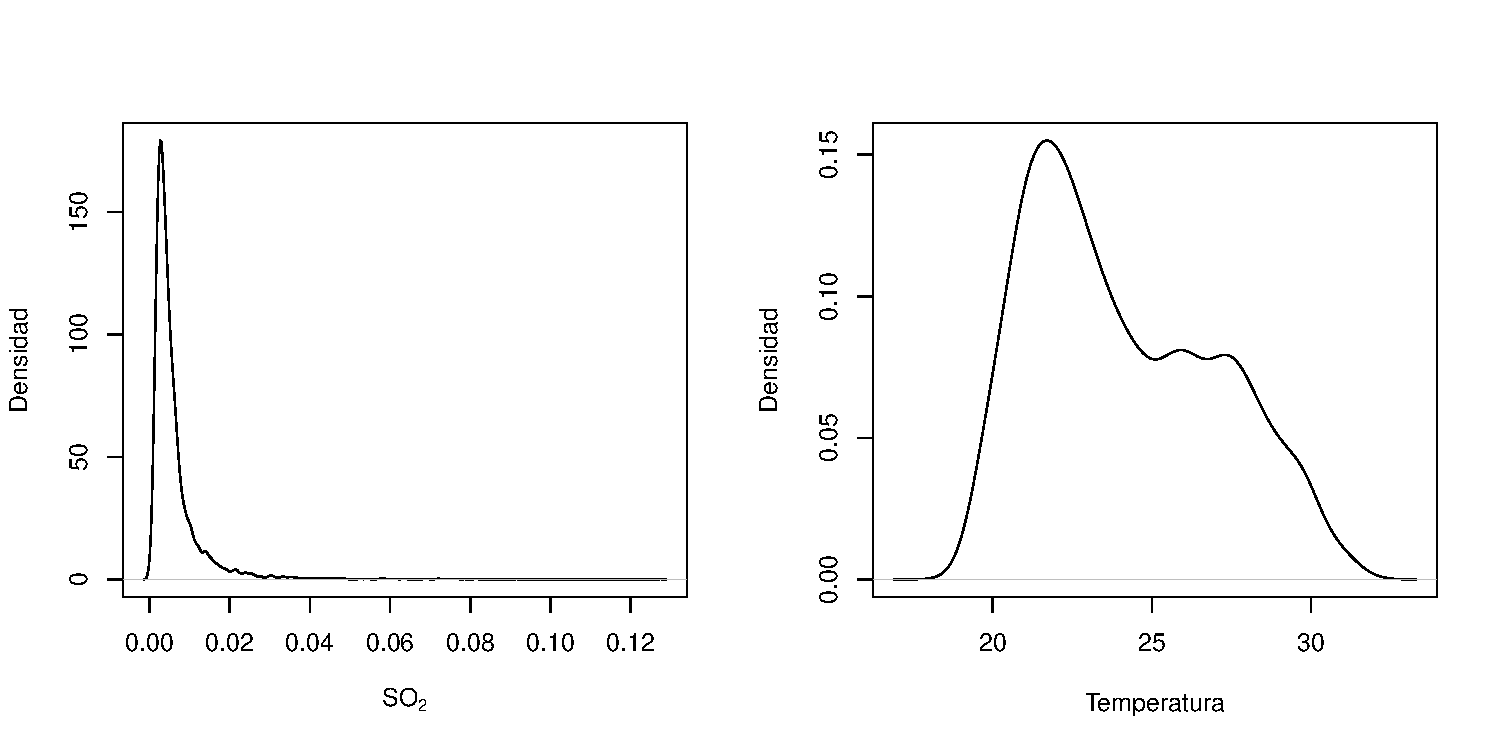
\includegraphics[width=10cm]{Figuras/Figura1.pdf}
        \caption{Titulo de la figura}
        \label{fig:Densidad}
    \end{center}
\end{figure}
 
Para referenciar una figura, se utiliza el texto ``ref'' precedido de un \textit{backslash}: as�, se referenciar�a la Figura \ref{fig:Densidad}.
\\
\\
Expresi�n matem�tica en l�nea con el texto: $f(x):=ax^2+bx+c$.
\\
\\ 
Representaci�n de una ecuaci�n, sin n�mero de referencia:
 
$$y_{i} = \beta_{0} + \beta_{1}x_{i} + \epsilon_{i}$$
 
Representaci�n de una ecuaci�n en una l�nea nueva, con n�mero de referencia:
 
\begin{equation}
 \bar{X} = \sum_{i=1}^{n}\frac{x_{i}}{n}
 \label{eq:media}
\end{equation}
 
Pare referenciar la ecuaci�n \eqref{eq:media}. Se utiliza la etiqueta ``eqref'' precedido de un \textit{backslash}
\\
\\
Para referenciar una cita bibliogr�ficas se utiliza un archivo ``Bibliografia.bib''. Este contiene la informaci�n de las referencias utilizadas. Por ejemplo para citar dentro del texto: Seg�n \cite{seber2012linear} plantea que el modelo de regresi�n.....

\subsection{}
 
$\left(\frac{365}{3}\right) \cdot \left(\frac{365}{4}\right) $
 
Una lista: 
 
\begin{itemize}
 \item primer �tem de la lista.
 \item segundo �tem de la lista.
\end{itemize}
 
Numeraci�n de una lista:
 
\begin{enumerate}
\item primer �tem de la lista.
\item segundo �tem de la lista.
\end{enumerate}


 
Ejemplo para construir una matriz:
 
$$I = \left[
\begin{array}{c c c c c}
        1    &    0    &    0    &    0    \\
        0    &    1    &    0    &    0    \\
        0    &    0    &    1    &    0    \\
        0    &    0    &    0    &    1
\end{array} \right]$$
 
% Insertar una gran cantidad de comentarios (bloque)
\begin{comment}
Este texto, al igual que aquel que est� precedido por un signo de porcentaje, no ser� mostrado en el documento final.
\end{comment}

\subsection{Scripts R}
El ambiente \emph{Verbatim} permite agregar codigo de R.
\begin{verbatim}
getwd()
k=70
cumpledif=1
p=0
q=0
for (j in 1:k){
  cumpledif=cumpledif*(1-((j-1)/365))
  q[j]=cumpledif
  p[j]=1-cumpledif
  cat(cumpledif,"\n")
}

windows()
pdf("Texmaker/Graficos/Punto2.pdf")
par(mfrow=c(1,3))
plot(p,col="red", xlab = "n", ylab = "Probabilidad", main = "Probabilidad de que dos o mas estudiantes 
tengan el mismo cumplea�os en funcion 
     de la cantidad de estudiantes n")
abline(h=0.5)
abline(v=23)

plot(q,col="blue", xlab = "n", ylab = "Probabilidad", main = "Probabilidad de que dos o mas estudiantes 
NO tengan el mismo cumplea�os en funcion 
     de la cantidad de estudiantes n")
abline(h=0.5)
abline(v=23)

plot(p,col="red", xlab = "", ylab = "")
par(new=TRUE)
plot(q,col="blue", xlab = "", ylab = "")

title(xlab = "n", ylab = "Probabilidad",main="Probabilidades de que dos o mas estudiantes 
tengan el mismo cumplea�os (rojo) y su 
evento complemetario (azul) en funcion de n")
dev.off()

###########simulacion punto 3a Exponencial

U = runif(1000, 0, 1) #Generar U
l = 4 #Par�ametro de la exponencial Lambda = 4
X = -(1/l) * log(U)
windows()
pdf("Texmaker/Graficos/Punto3A.pdf")
par(mfrow=c(1,2))
plot(density(U),col="blue", xlab = "X", ylab = "Densidad", main = expression(Unif(0,1)))
plot(density(X),col="red", xlab = "X", ylab = "Densidad", main = expression(Exp(lambda=4)))
dev.off()

############ Punto 3b Poisson 
x=0
for(j in 1:1000){
  lambda=7
  i = 0
  p = exp(-lambda)
  f = p
  u= runif(1000,0,1)
  while(u>=f){
    p=lambda*p/(i + 1)
    f = f + p
    i = i +1
    x[j] = i
  } 
}

\end{verbatim}


\subsection{Analisis Resultados}


\section{Situacion 2}
\subsection{Punto A.}
~\\\textbf{Si $\hat{\theta_1}$ y $\hat{\theta_2}$ son dos estimadores insesgados tales que:
~\\$$\hat{\theta_3}=a{\hat{\theta_1}}+(1-a){\hat{\theta_2}}$$}
~\\ Aplico Esperanza a ambos lados 
~\\ $E[\hat{\theta_3}] = E[a{\hat{\theta_1}}+(1-a){\hat{\theta_2}}]$
~\\ $E[\hat{\theta_3}] = E[a{\hat{\theta_1}}]+E[(1-a){\hat{\theta_2}}]$
~\\ $E[\hat{\theta_3}] = E[a{\hat{\theta_1}}]+(1-a)E[{\hat{\theta_2}}]$ \textbf{Con $\hat{\theta_1}$ y $\hat{\theta_2}$ estimadores insesgados}\
~\\ $E[\hat{\theta_3}] = a{\theta} + (1-a){\theta}$
~\\ $E[\hat{\theta_3}] = a{\theta} + {\theta} - a{\theta}$
~\\ $$E[\hat{\theta_3}]={\theta}$$

~\\\textbf{$\therefore \hat{\theta_3}$ Es un estimador insesgado.} 
 


\subsection{Punto B.} 

~\\\textbf{ El coeficiente de variacion de $\hat{\theta_3}$ es}
~\\
~\\ $$CV[\hat{\theta_3}]=\frac{\sqrt{Var[\hat{\theta_3}]}}{E[\hat{\theta_3}]}$$
~\\ Hallamos la $Var[\hat{\theta_3}]$
~\\ $Var[\hat{\theta_3}]=Var[a{\hat{\theta_1}}+(1-a){\hat{\theta_2}}]+2Cov[a{\hat{\theta_1}},(1-a){\hat{\theta_2}}]$,    ya que no sabemos si ${\hat{\theta_1}}$ y ${\hat{\theta_2}}$ son independientes
~\\ Entonces, distribuyendo la Varianza y por las propiedades de Covarianza:
~\\ $Var[\hat{\theta_3}]=Var[a{\hat{\theta_1}}]+Var[(1-a){\hat{\theta_2}}]+2a(1-a) Cov[{\hat{\theta_1}},{\hat{\theta_2}}]$
~\\ $Var[\hat{\theta_3}]=a^2Var[{\hat{\theta_1}}]+(1-a)^2Var[{\hat{\theta_2}}]+(2a-2a^2)Cov[{\hat{\theta_1}},{\hat{\theta_2}}]$
~\\
~\\\textbf{Como $Var[{\hat{\theta_1}}]=\sigma_1^2$ y $Var[{\hat{\theta_2}}]=\sigma_2^2$ entonces}

~\\ $Var[\hat{\theta_3}]=a^2[\sigma_1^2]+(1-a)^2[\sigma_2^2]+(2a-2a^2)Cov[{\hat{\theta_1}},{\hat{\theta_2}}]$
~\\ Sabemos que $Cov[{\hat{\theta_1}},{\hat{\theta_2}}]= E[{\hat{\theta_1}}{\hat{\theta_2}}]- E[{\hat{\theta_1}}]*E[{\hat{\theta_2}}]$, entonces:
~\\ Como $E[{\hat{\theta_1}}]={\theta}$ y $E[{\hat{\theta_2}}]={\theta}$ tenemos:
~\\ $Cov[{\hat{\theta_1}},{\hat{\theta_2}}]=E[{\hat{\theta_1}}{\hat{\theta_2}}]-{\theta^2}$, por tanto:
~\\ $Var[\hat{\theta_3}]=a^2[\sigma_1^2]+(1-2a+a^2)[\sigma_2^2]+(2a-2a^2)(E[{\hat{\theta_1}}{\hat{\theta_2}}]-{\theta^2})$
~\\ Como sabemos que $E[\hat{\theta_3}]={\theta}$

~\\$\therefore$ \textbf{El coeficiente de variacion para $\hat{\theta_3}$ es:}  
$$CV[\hat{\theta_3}]=\frac{\sqrt{a^2\sigma_1^2+(1-a)^2\sigma_2^2+(2a-2a^2)(E[{\hat{\theta_1}}{\hat{\theta_2}}]-{\theta^2})}}{{\theta}}$$

\subsection{Punto C.} 
~\\ Como en este punto sabemos que $\hat{\theta_1}$ y $\hat{\theta_2}$ son independientes, entonces la $Cov[{\hat{\theta_1}},{\hat{\theta_2}}]=0$ y por tanto:
~\\ $Var[\hat{\theta_3}]=Var[a{\hat{\theta_1}}+(1-a){\hat{\theta_2}}]$
~\\ Distribuyendo la varianza y aplicando sus propiedades, nos queda:
~\\ $Var[\hat{\theta_3}]=Var[a{\hat{\theta_1}}]+Var[(1-a){\hat{\theta_2}}]$ 
~\\ $Var[\hat{\theta_3}]=a^2Var[{\hat{\theta_1}}]+(1-a)^2Var[{\hat{\theta_2}}]$
~\\ $Var[\hat{\theta_3}]=a^2\sigma_1^2+(1-a)^2\sigma_2^2$ 
~\\ Note que $Var[\hat{\theta_3}]$ se convierte en una funcion que depende de a, ya que, $\sigma_1^2$ y $\sigma_2^2$ son conocidas, entonces, debemos encontrar a, que haga minima dicha funcion, en otras palabras, todo se reduce a encontrar el minimo de la funcion. Para ello procedemos de la siguiente manera:
~\\ 1. Encontramos la primera derivada de la funcion con respecto a la variable a:
~\\ $$f'(a)=2a\sigma_1^2 - 2(1-a)\sigma_2^2$$
~\\ 2. Igualamos el resultado de la primera derivada a 0 y despejamos la variable que nos interesa obtener, en este caso, despejamos a:
$$2a\sigma_1^2 - 2(1-a)\sigma_2^2=0$$
$$2a\sigma_1^2 - (2-2a)\sigma_2^2=0$$
$$2a\sigma_1^2 - 2\sigma_2^2 + 2a\sigma_2^2=0$$
$$2a\sigma_1^2  + 2a\sigma_2^2= 2\sigma_2^2$$
$$a(2\sigma_1^2+2\sigma_2^2)=2\sigma_2^2$$
$$a=\frac{2\sigma_2^2}{2\sigma_1^2+2\sigma_2^2}$$
~\\$\therefore${$a=\frac{\sigma_2^2}{\sigma_1^2+\sigma_2^2}$}
~\\ 3. Ahora, debemos encontrar la segunda derivada y ver si es positiva o negativa para saber si encontramos un minimo o un maximo:
~\\$$f^{\prime\prime}(a)=2\sigma_1^2+2\sigma_2^2 > 0$$
~\\ Como nos dio que la segunda derivada parcial es siempre positiva, concluimos que el a hallado anteriormente es un minimo. Por lo tanto, para hacer que la $Var[\hat{\theta_3}]$ sea minima, debemos escoger a como $a=\frac{\sigma_2^2}{\sigma_1^2+\sigma_2^2}$.

\section{Situacion 3}
\subsection{Punto A.}

Sea $X$ una distribucion Poisson$(\lambda)$ con, $n=30$ y $E[x]=(\lambda)$

$$\ M'_1 = \frac{1}{30} \sum_{i=1}^{30}x_{i}$$
$$\ M'_1 = (\lambda)$$

$$\ M'_1 = \frac{1}{30} \sum_{i=1}^{30}x_{i} = \lambda = M'_1$$

$$\therefore \hat{\lambda}= \frac{1}{30} \sum_{i=1}^{30}x_{i} = \overline{X}$$
 
~\\Ahora es necesario probrar si es insesgado: 

$$E[\hat{\lambda}]=E[\frac{1}{30} \sum_{i=1}^{30}x_{i}]$$
$$E[\hat{\lambda}]=\frac{1}{30} E[\sum_{i=1}^{30}{\lambda}_{i}]$$
$$E[\hat{\lambda}]=\frac{1}{30}30\lambda$$
$$E[\hat{\lambda}]=\lambda$$

~\\$\therefore$ \textbf{Un estimador insesgado para} $\lambda$ \textbf{es} $\hat{\lambda}= \frac{1}{30} \sum_{i=1}^{30}x_{i} = \overline{X}$

\subsection{Punto B.}

Sea $C=3X+X^2$

$$E[C]=E[3X+X^2]$$
$$E[C]=E[3X] + E[X^2]$$
$$E[C]=3E[X] + E[X^2]$$

~\\ Sabiendo que:
 
$$V[X]=E[X^2] - E^2[X]$$


~\\ Entonces: 

$$E^2[X] = V[X] + E[X^2]$$

~\\$$\therefore E^2[X] = \lambda + (\lambda)^2$$

~\\ Reemplazando $E^2[X]$ en:\ 

$$E[C]=3\lambda + E[X^2]$$

~\\Obtenemos que: 
$$E[C]=3\lambda + \lambda + (\lambda)^2$$
$$\therefore E[C] = 4\lambda + (\lambda)^2$$


% Bibliografia utilizada 
\bibliography{Bibliografia}
\end{document}